\chapter{Implementation}
\label{cha:impl}

In this chapter I will outline the entire process, detailing how I went from a raw dataset, to the final application displaying hotspots with Leaflet.

\section{Pre-Processing}

Figure \ref{bbdatatable} showed the raw format of the Britain Breathing dataset. There are a few procedures that need doing before it can be used in a hotspot identification algorithm.\\

The Britain Breathing dataset contained entries from all over the world. I could have left these entries in such that a curious user could pan the map to those areas of the globe. However, I decided to remove all points not on mainland UK or in Northern and the Republic of Ireland as they would affect global averages and therefor affect hotspot calculations.

The Britain Breathing dataset in its raw format contained entries from all over the world. I could have decided to leave them in as I could centre the map on the UK so that only those who were curious enough to pan around the rest of the globe would see these extra points. But that's more of a novel addition. At the time of pre-processing, I thought the extra points might affect some of the hotspot algorithm calculations such as global averages so I decided to remove all points that are not on mainland UK or in Northern and the Republic of Ireland.\\

\begin{figure}[H]
\begin{center}
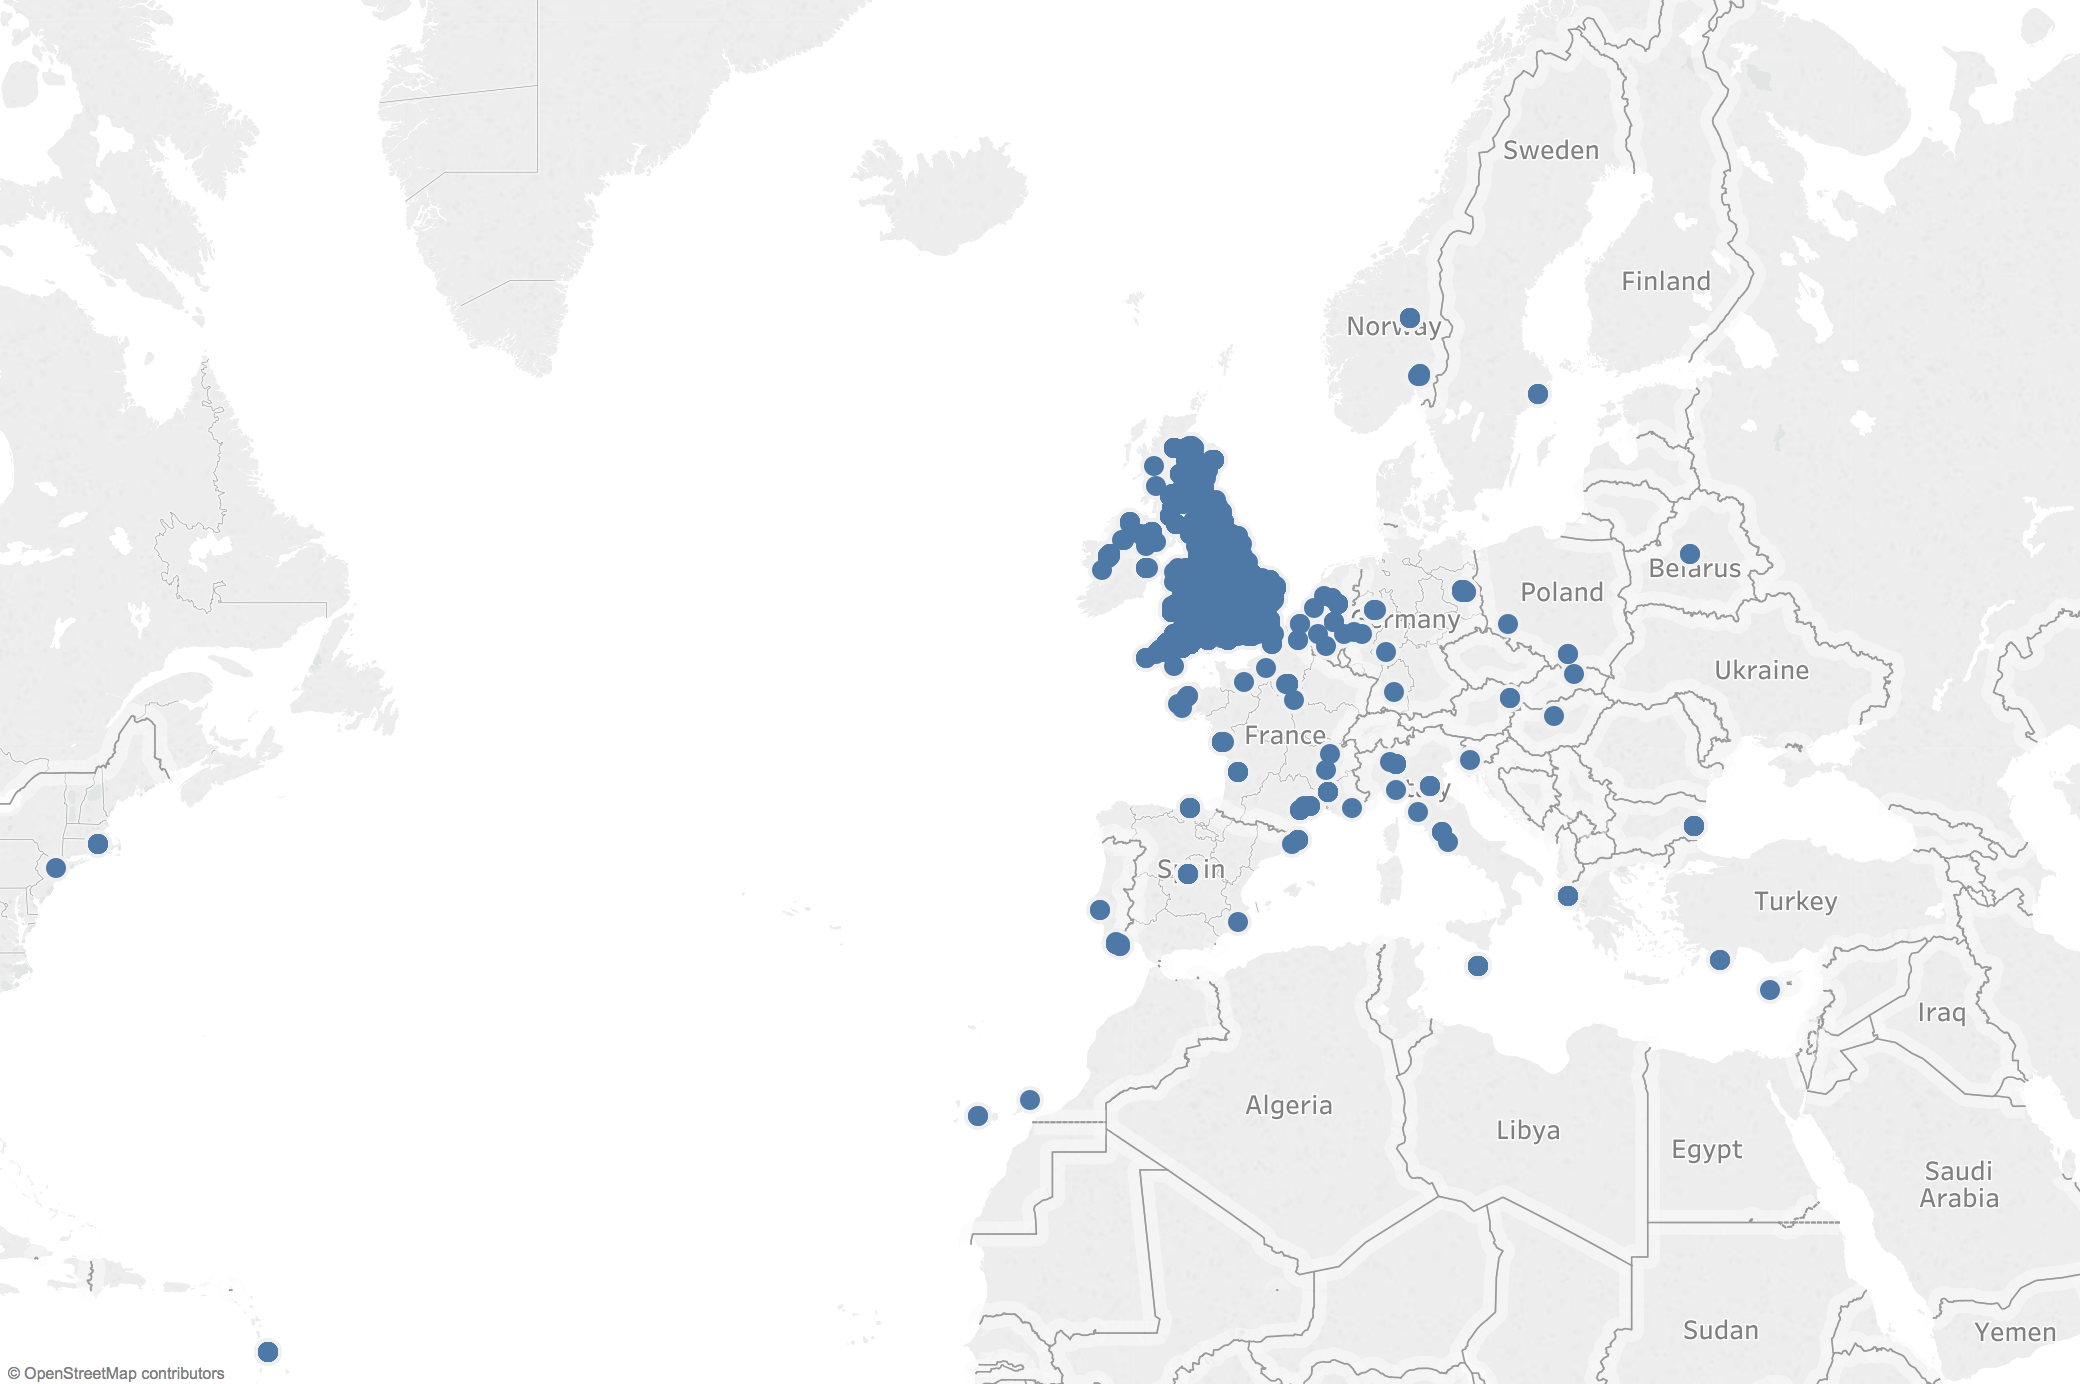
\includegraphics[width=0.75\textwidth]{tableuaeverywhere}
\caption{Britain Breathing dataset before processing}
\label{fig:RTv1}
\end{center}
\end{figure}

Approximately 2.7\% of entries had a null value for one of the attributes, I assume because they were not asserted as being necessary in the data collection application. 96\% of these nulls were  whether the user had existing hay fever or asthma, I decided to remove each of these records entirely. Although the attribute could have been set to 0 or 1 for all entries, I wanted to avoid fabricating data to keep any conclusions made using the data valid.


I could have decided set the attribute to 0 or 1 for all entries but I wanted to avoid fabricating data to keep any conclusions made using the data valid.\\

Whilst using Tableau to visualise the data in the early stages of development, I noticed there were a few clusters of points in close proximity. For example, there was a user in the north of Scotland who used the app at times multiple times per day to record their allergy symptoms. This resulted in a fairly large set of results for a very sparsely populated area. I decided to remove most of these results as the area was identified as a hotspot. Thereis an argument for keeping the data, but I don't believe that including one person's enthusiasm to track their allergy problems makes sense for a project aimed at producing results that could be used to aid research.\\

Once the data was improved from its raw format, it was stored on the server as a JSON file. I decided against using a database to store my datasets as I wanted to avoid having to convert to and from JSON. The end application ended up being rather CPU intensive at times so this proved to be useful.

\subsection{Road Traffic}

The Road Traffic dataset required significantly more processing to become usable. As is evident from figure \ref{fig:rt}, the first version of the Road Traffic dataset was far too dense. I needed the Road Traffic dataset to be able to be viewed on top of the Britain Breathing dataset in order to compare and contrast. There were too many roads with very short spans cluttering the view of the heatmap.\\

\begin{figure}[H]
\begin{center}
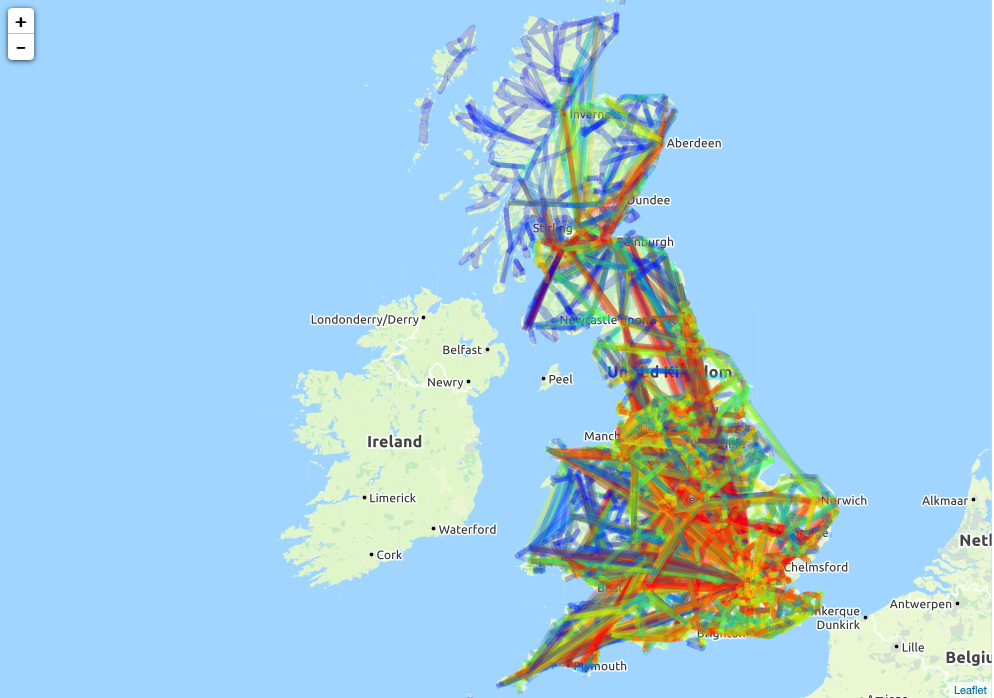
\includegraphics[width=1\textwidth]{RoadTrafficv1}
\caption{First attempt at displaying the Road Traffic data. Requires filtering to be viewable.}
\label{fig:rt}
\end{center}
\end{figure}

Upon zooming in and inspecting the data, I also found that some roads were stored incorrectly in the dataset. Ten roads were stored as having their junction before and junction after the count point as being the ends of the road. Roads like the A1 are as long as 396 miles, so these types of errors can cause incorrect representations of data \cite{longestRoad}. In the case of the A1, the entire road was displayed as a deep red, indicating a high volume of traffic. For the majority of the A1, this would be true but there are areas of the road that are not especially busy, so they are  wrongly represented.\\

I created a Java program to process the data before being stored on the server. Java was chosen because I have most experience with it, I knew exactly how to read and write files, making it a good choice for pre-processing the Road Traffic data. For each record, counts are discarded if the length of the distance between the junction before and the junction after is longer than 200km, or if the road is shorter than 5km and has a density in the lower 5\% of the data. Removing the smaller roads like this removes the mess of small roads with negligible traffic in places such as the north of Scotland. These roads don't provide much information and therefore do not help to find hotspots, they just make the map look cluttered.\\

\subsection{Analysis Field}
\label{sec:anal}

The Britain Breathing dataset has many attributes that are relevant to allergy symptoms.\\

\begin{table}[H]
\begin{tabular}{|c|c|c|c|}\hline\hline
Attribute&Represents&Range&Range Description\\\hline
how\_feeling&General well-being of the person&0..2&0 Best, 2 Worst\\
breathing&Condition of lungs and trachea&0..2&0 Best, 2 Worst\\
eyes&Condition of the eyes&0..2&0 Best, 2 Worst\\
nose&Condition of the nose&0..2&0 Best, 2 Worst\\
hayfever&Suffers from hay fever&0..1&0 no, 1 yes\\
asthma&Suffers from asthma&0..1&0 no, 1 yes\\
taken\_meds\_today&Taken allergy medication&0..1&0 no, 1 yes\\\hline\hline
\end{tabular}
\caption{Britain Breathing Dataset Allergy Related Attributes. 13 attributes removed for simplicity}
\label{bbdata}
\end{table}

All of the attributes within Figure \ref{bbdata} contribute to the overall severity of a persons allergy symptoms on any given day. In order to use with hotspot identification algorithms, there needs to be a single attribute that is a summary of the others. They all must be combined into one value that can be used to indicate a records Allergy Score, or more generically so that it fits the Road Traffic dataset too, the Analysis Field.\\

In the development of the Analysis Field for the Britain Breathing dataset, I made some initial judgements and then adjusted the parameters with some trial and improvement. The Analysis field needs to be a summary of the others. Keeping this in mind, I assigned a high priority to the how\_feeling attribute as it itself is a summary of the persons general allergy related feeling. I then assigned breathing, nose and eyes with roughly similar weightings. I used the taken\_medication\_today as a multiplier for the breathing, nose and eye symptoms using the reasoning that if a person has taken their medication and is still suffering, then they should score higher than someone with the same values for the other attributes but has not taken their medication. Hay fever and asthma attributes are used, but do not have much of an effect on the Analysis Field.\\

$Analysis Field (AF) = 2*(how\_feeling*(0.5*nose + 0.3*eyes + 0.3*breathing)) + \\(taken\_meds\_today*(nose + eyes + breathing)) + asthma + hayfever$\\

The above formula is used to calculate the Analysis field in the final version of Inhale. It seems to work well, I'm happy it uses a wide spread of attributes but still focuses on the main four; how\_feeling, nose, breathing and eyes.\\

The Analysis field for the Road Traffic dataset was simpler. To keep the field relevant to allergies, I decided to focus on the emissions from vehicles on that road per hour. At first I simply found that the average $CO_2$ emissions for a combustion engine vehicle was 411 g/mile or 274g/km and I multiplied the total traffic count by this value \cite{trafficemiss}. The traffic counts were not anywhere near perfectly distributed. Different roads had very different distributions of vehicle types. For example, the two main corridors between the North and South of England, the M6 on the East and the A1 on the West both had far higher percentages of HGV type vehicles than the average road.\\

With the disparity in vehicle distribution in mind, I found the average vehicle emissions for each vehicle type instead. Then simply created the Analysis Field as below.

\begin{myequation2}%
Analysis Field (AF) = \sum_{vt=1}^n VehicleCount * VehicleTypeEmissions
\end{myequation2}

As previously mentioned, the dataset is not entirely consistent with its junctions before and after the counting point. Although I removed the problematic roads, there could be many more less obvious roads with similar problems. Ideally, the vehicle emissions per km would be used and that would be multiplied that by the distance between the junction before and after to get a total emission value for the vehicle. Unfortunately, not only would this not be possible due to the problems in the dataset, but it would also produce useless results. It does not matter how far a vehicle has travelled on its way to you, only the distance it has travelled in a small radius around you should be considered as this is the area in which its emissions can reach affect you.\\

As a compromise, I simply used the g/km value as a measure of it's emissions without taking into account the actual number of km travelled by that vehicle. This could perhaps be improved by calculating the distance of the road that is within x km of the user.

\section{Heatmap Generation}

Once the data is in a usable format and condition, I need to display that data on a map. In this section will explain the steps taken to get to point where I have a allergy symptom hotspots represented as a heatmap using Leaflet.\\

The Britain Breathing JSON file is loaded from the server. An instance of a HotspotArray is instantiated with parameters including x and y values for the dimension of the desired map resolution. The resolution values are used to create a two dimensional array with sizes [x][y]. This array is used to divide the area of the UK into distinct square areas. See figure \ref{fig:hh} for a small scale example.

\begin{figure}[H]
\begin{center}
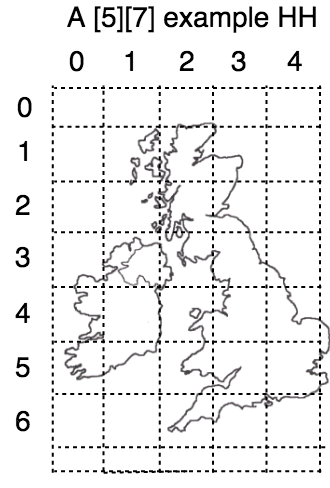
\includegraphics[width=0.4\textwidth]{hh5x7}
\caption{A [5][7] resolution example}
\label{fig:hh}
\end{center}
\end{figure}

By default, I used a 500 by 500 resolution as I found this gives enough of a resolution so that you can't see the square boundaries at any zoom level but also keeps the calculations running quickly enough to give a smooth use experience. The alternative here would have been to use something like the UK Council boundaries, but I didn't like how they looked on the map, mainly due to the fact that dividing the map by Councils meant that you don't get precise enough information on specific allergy symptoms hotspots. A hotspot in a City such as Inverness would cause the entire massive Scottish Highlands council district to be indicated as being a hotspot. The Scottish Highlands has many very small villages, some with as few as three or four houses, so this would likely create many false hotspots.\\

For each entry in the dataset;

\begin{enumerate}
    \item Add entry to the Hotspot Array. The latitude and longitude of the entry is used to map to an index in the array. For example, a location in the top left of the map would map to [0][0], bottom right would map to [499][499] etc. 
    \item If there is already a value in the Hotspot Array, add to the total count and update the average for the square area. Otherwise, add to the total count and calculate average.
\end{enumerate}

The next step after filling the Hotspot Array with the data is to do some hotspot identification.

\subsection{Spatial Autocorrelation}

Determining if an area is a hotspot or not can be done using Spatial Autocorrelation (SA). SA is a way of giving a numerical value to the degree of which an area is similar to nearby areas \cite{autocor}. SA algorithms usually provide a z-score for an area, a high positive z-score indicates that an area has a statistically significant value when compared to its neighbours and should be indicated as a hotspot as it is a cluster of high values. A low positive or low negative value indicates that it is likely that the value is randomly clustered. A high negative value shows a cluster of low values. See Figure \ref{fig:autocor2} for a diagrammatic description.\\

\begin{figure}[H]
\begin{center}
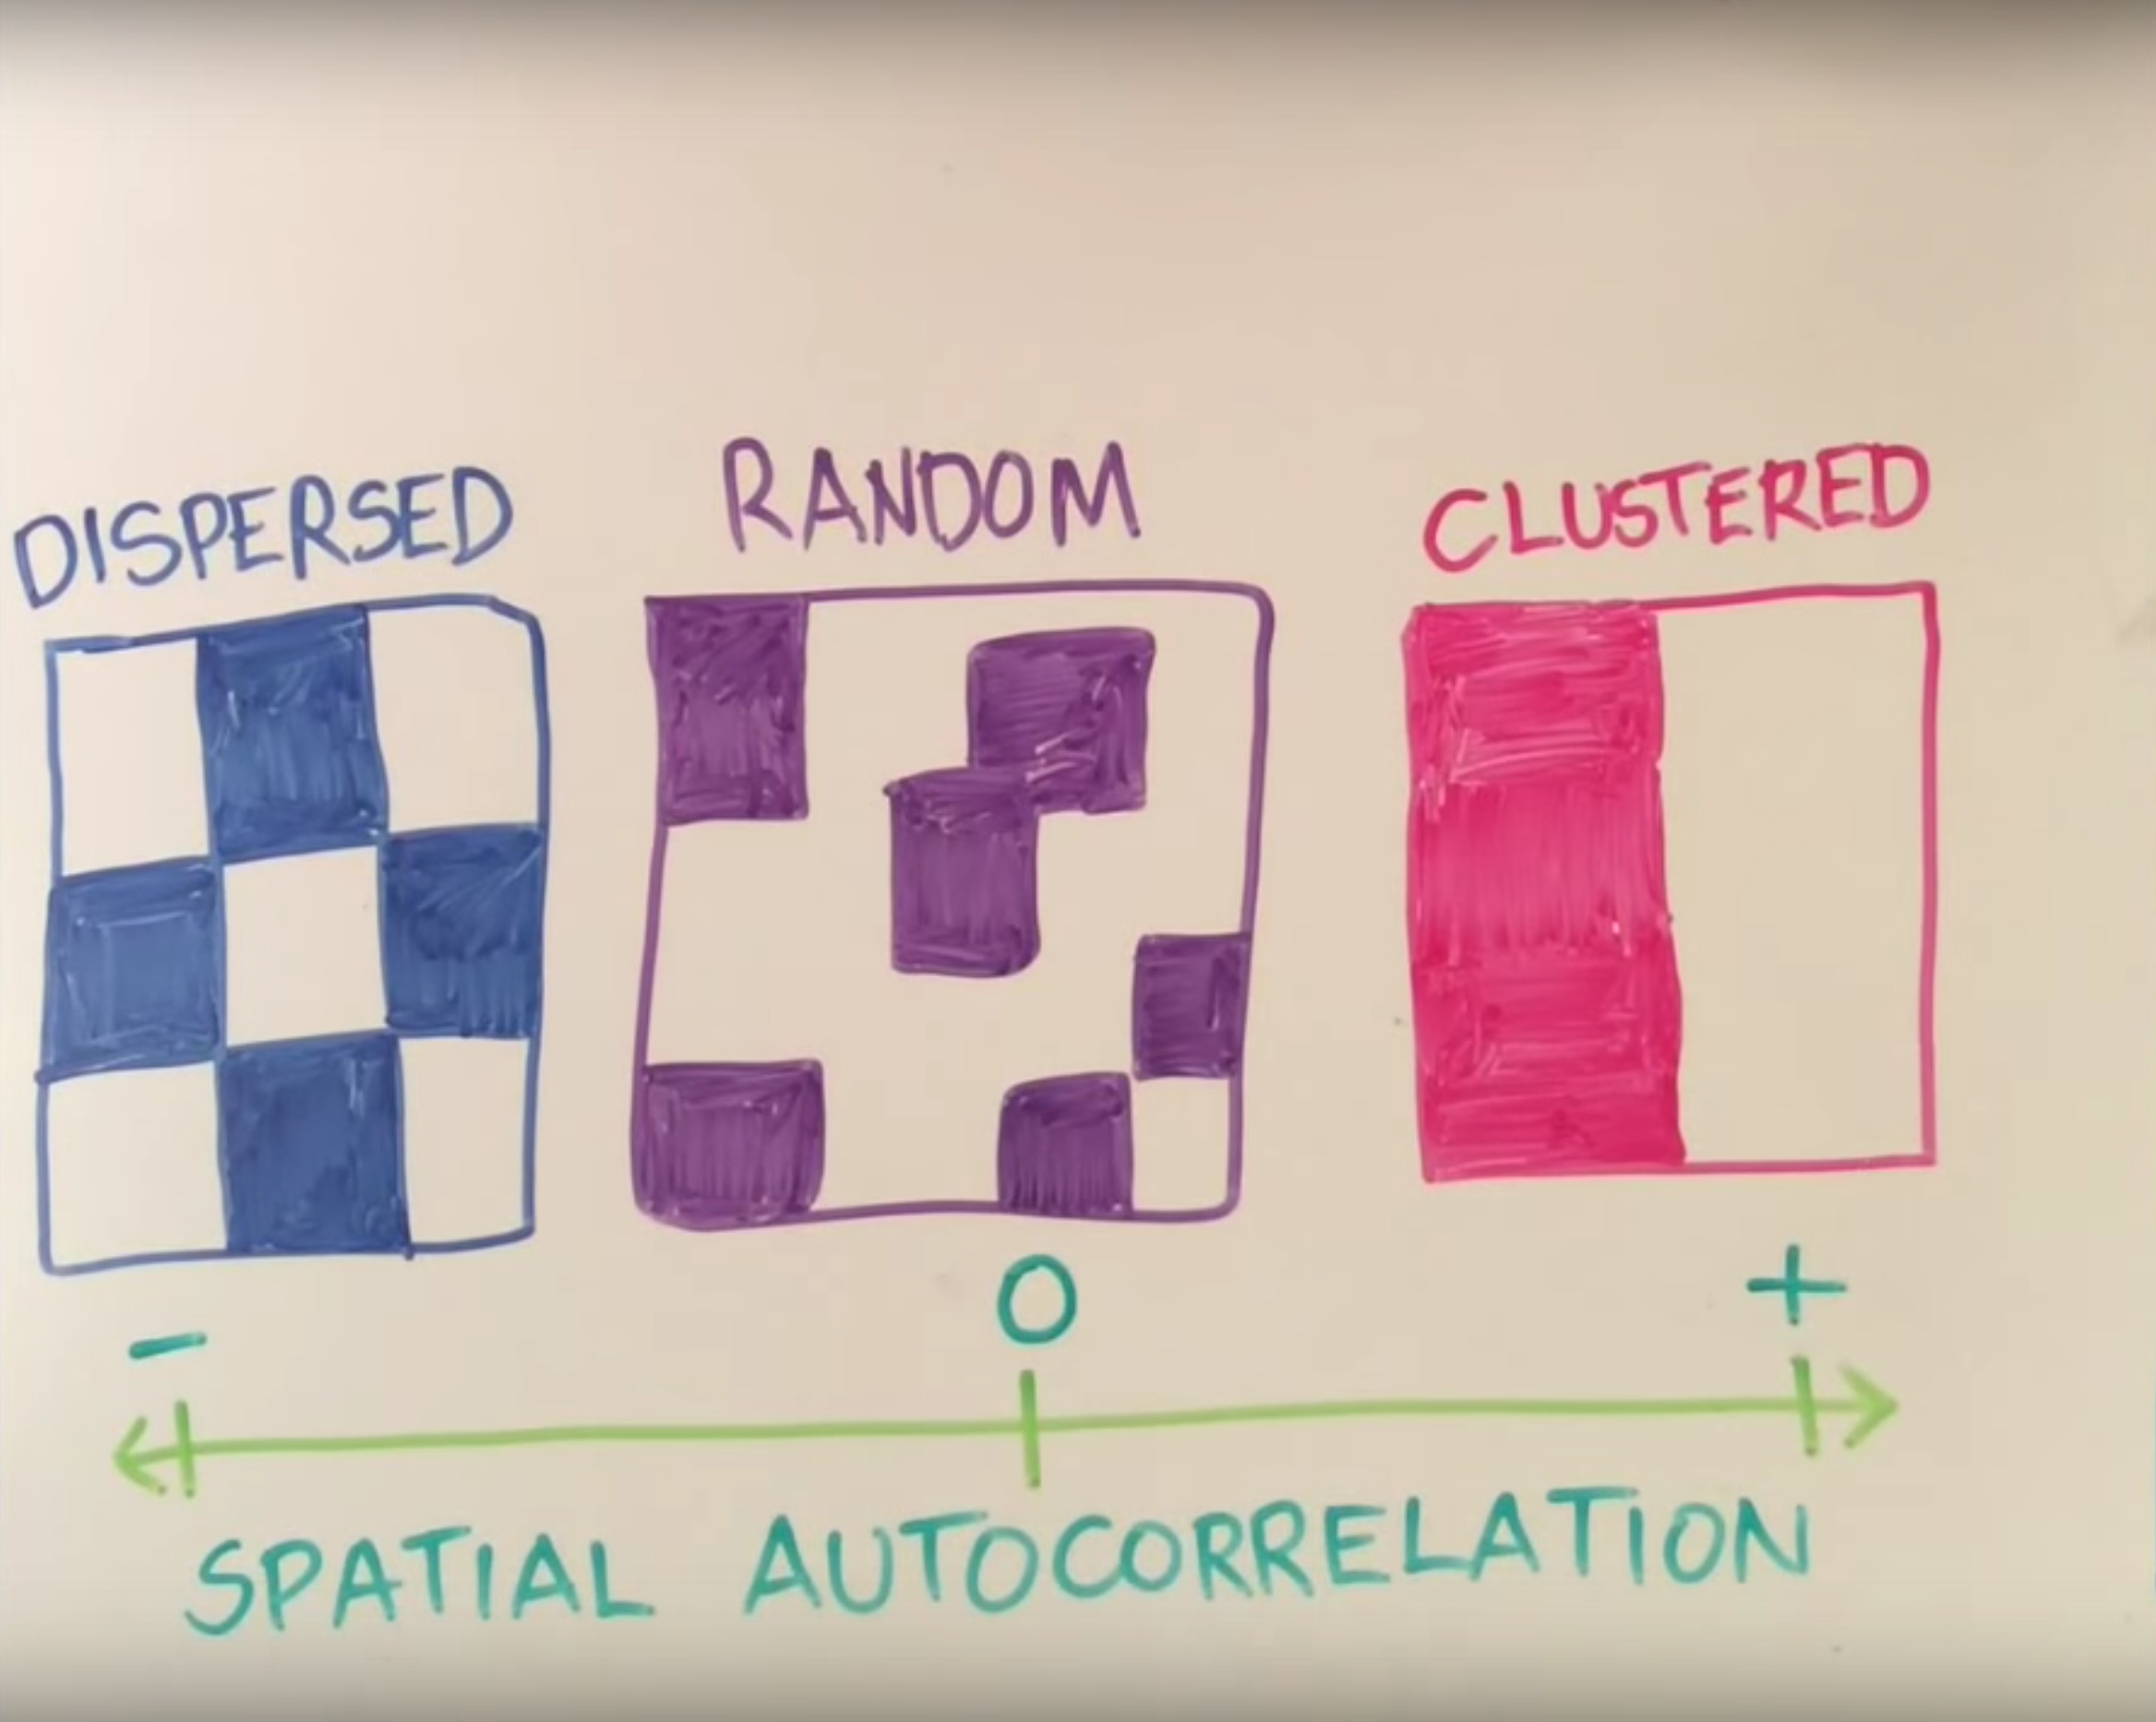
\includegraphics[width=0.8\textwidth]{autocor2}
\caption{Correlation Types \cite{ytcorr}}
\label{fig:autocor2}
\end{center}
\end{figure}

If an area has a high positive value then we can consider that area a hotspot, therefore, if an array entry has lots of high positive values they should accumulate to generate a higher allergy symptom score. Equally, if an area has a few high positive values, a few small absolute values and a few large negative values, the algorithm should take this into account and not label the area as a hotspot.\\

An effective way of doing this is to take an average of the z-scores for the area, then use the average in the heatmap.

\subsection{Distance Calculations}

Calculating the statistical significance of values, and whether or not they are related to nearby values requires calculating the distance between points.\\

There are many ways of calculating the distance between a pair of two dimensional points, namely Euclidean and Manhattan. Euclidean is the straight line distance between two points and Manhattan is the distance when navigating in a grid like manor \cite{manhatc}. Choosing between these distance calculation methods is not particularly important as they would both produce similar results, I chose Manhattan distance for this project, the mathematical equation is presented in Figure \ref{dia:manhat}

\begin{figure}[h]
\begin{center}
$dist (x, y)  = \sqrt{\sum_{i=1}^n (x_i - y_i)^2 }$
\caption{Manhattan Distance}
\label{dia:manhat}
\end{center}
\end{figure}

\subsection{Using distances}

The closer two points are, the more they will affect each other. It would not be correct to say that a cluster of allergy symptoms in Manchester would have any affect at all on those in Liverpool. So a way of using these distances to calculate how much to take the surrounding areas into account is needed. Waldo Tobler's first law of Geography describes this succinctly, "everything is related to everything else, but near things are more related than distant things." \cite{waldo}\\

The focus of this project is on the symptoms  of allergies; most allergen producers do not have a method of mass dispersion. What I mean by this is they do not have a way of dispersing the produced allergens significant distances. Around 2km is normal, with the largest known distance being 21km travelled by some Bentgrass pollen on a windy day in the US \cite{pollenwr}. I can use this fact because I want to make sure that my hotspots are location specific and don't take into account any allergen producers over 20km because the chances are that allergens produced by them haven't reached the area.\\

The length of the entire UK is around 874 miles, with the length of the visible map in Inhale being 1000 miles. Divide 1000 by 500 and you get 2 square miles per HotspotArray entry. This means that the average point in an area has a distance of 2 miles to the average point in the area directly to the left, right, up or down. When comparing to neighbouring areas, I want to consider the area directly next to the area in question, and perhaps only very slightly consider the areas one square further than those, just to account for other types of allergens which may travel further.\\

I decided to use a inverse distance weighting with a strong fall off for neighbouring areas. See Figure \ref{table:dist} for the calculations used to determine the inverse distance function. I decided to use $\frac{1}{x^3}$ as it has the right amount of drop off for distances of three or squares away but still uses areas of distance two with a 0.125 factor.\\ 

\begin{table}[H]
\begin{center}
\begin{tabular}{|c|c|c|c|}\hline\hline
x&$\mathbf{\frac{1}{x^2}}$&$\mathbf{\frac{1}{x^3}}$&$\mathbf{\frac{1}{x^4}}$\\\hline
1&1&1&1\\
2&0.25&0.125&0.0625\\
3&0.111&0.037&0123\\
4&0.0625&0.0156&0.0039\\\hline\hline
\end{tabular}
\caption{Potential Inverse Distance Functions}
\label{table:dist}
\end{center}
\end{table}


\subsection{Getis-Ord}

Getis-Ord Gi* is a specific type of a spatial autocorrelation algorithm. I decided to use Gi* as the alternative solutions such as Morans-I tended not to include the feature being examined in the distance weightings. For this particular usage it is very important to include the immediate area within the square of the point being examined when calculating z-scores as allergen dispersion distances are so small.

Here's the equation;

\begin{myequation}%
Gi^* = \frac{\sum_{j=1}^{n} w_{i,j}x_{j} - \overline{X} \sum_{j=1}^{n} w_{i,j}}{{S \sqrt{\frac{n \sum_{j=1}^{n} w^2_{i,j} - (\sum_{j=1}^{n} w_{i,j})^2}{n-1}}}}
\end{myequation}

In summary, it takes the Analysis Field and compares it to every other point on the map using the inverse distance function making sure that distant areas have less effect on the resulting value. This is then used to determine whether or not the area is locally statistically significant and should be represented as a hotspot.

\subsection{Speed Issues and the Solution}

When calculating the Getis-Ord Gi* values for each area in the 500 by 500 array, you need to calculate the distance between that area and every other area. This quickly becomes a large problem of scale $O(n^2)$. Even though the distance calculations are very fast, the total time to run the Getis-Ord calculations was 14 seconds. As Inhale is hosted online and running using JavaScript, I must program such that any CPU can run Inhale quickly enough to be enjoyable.\\

The Britain Breathing dataset is displayed by default every time you load Inhale. Usually, no changes are made to the data and the Getis-Ord calculations are stable meaning the same input will always produce the same output. Each time the Getis-Ord z-scores are produces for a certain dataset, the results are stored in an array such that they do not have be calculated every time.\\

I implemented a cache system to speed up the process wherever possible. I designed the process with future updates in mind, where the user can change the base data and so Inhale is prepared to re-calculate the Getis-Ord z-scores if necessary.\\

The cache system is outlined below:\\

\begin{enumerate}
    \item Compute MD5 hash of input array
    \item Check if cache array contains an entry for the input
    \item \textbf{If contains entry} - pull the corresponding output array of z-scores. \textbf{Otherwise} - Compute Getis-Ord z-scores.
\end{enumerate}

When the cache finds an entry in the array and subsequently loads the output array instead of recalculating, the time taken plummets to an average of 0.12 seconds, a marked improvement over 14 seconds. This change was one of the simplest, but made one of the biggest differences to the usability of Inhale.

\section{Smart Data Tool}

The Britain Breathing dataset is displayed and the user can compare it to the Road Traffic set. I would have liked to have compared to more datasets, but there are not many good quality, relevant geographical datasets available online. The majority cost money or are entirely private. However, this should not stop Inhale from being used by those with access to those datasets from comparing their own sets to allergies.\\

I implemented a Smart Data Tool (SDT), to introduce the capability to upload your own dataset to be compared. The SDT can parse csv, tsv or JSON. For a dataset to be displayed on the map, it needs to have a location attribute. This is usually a Latitude/Longitude pair, or a Northing/Easting pair. SDT automatically detects these from the dataset and attempts to map them for the user.\\

The SDT also asks for a "Value Field", this is the field that will be used as the Analysis field in representations that require hotspot identification, or it can be used as a label in datasets that only require a simple marker for each entry. For example, in Figure \ref{fig:sdt}, the SDT has been used to upload the uk-towns-sample.csv dataset. It has automatically detected the Latitude and Longitude fields, and allows you to select an appropriate label for the marker tooltip to display when hovered over.\\

\begin{figure}[H]
\begin{center}
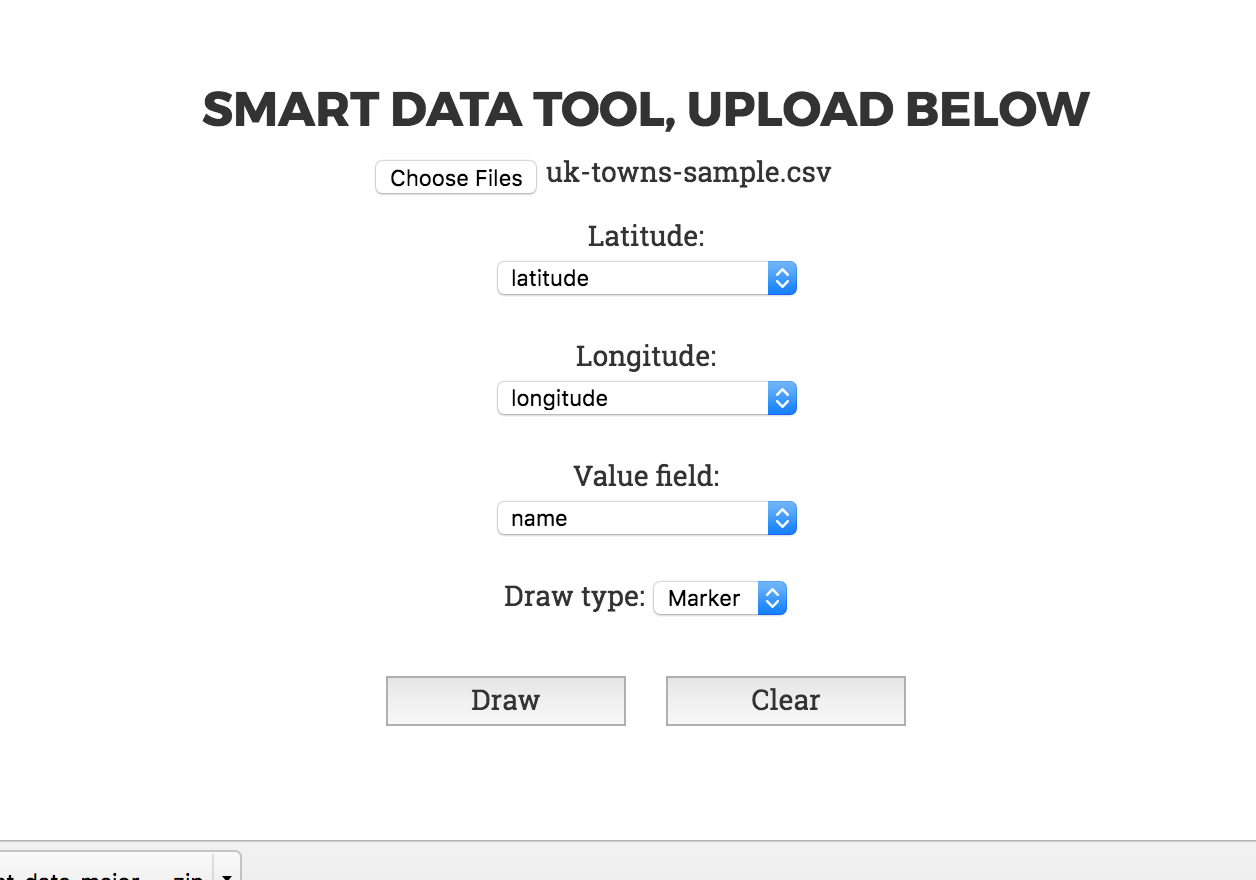
\includegraphics[width=0.4\textwidth]{sdt}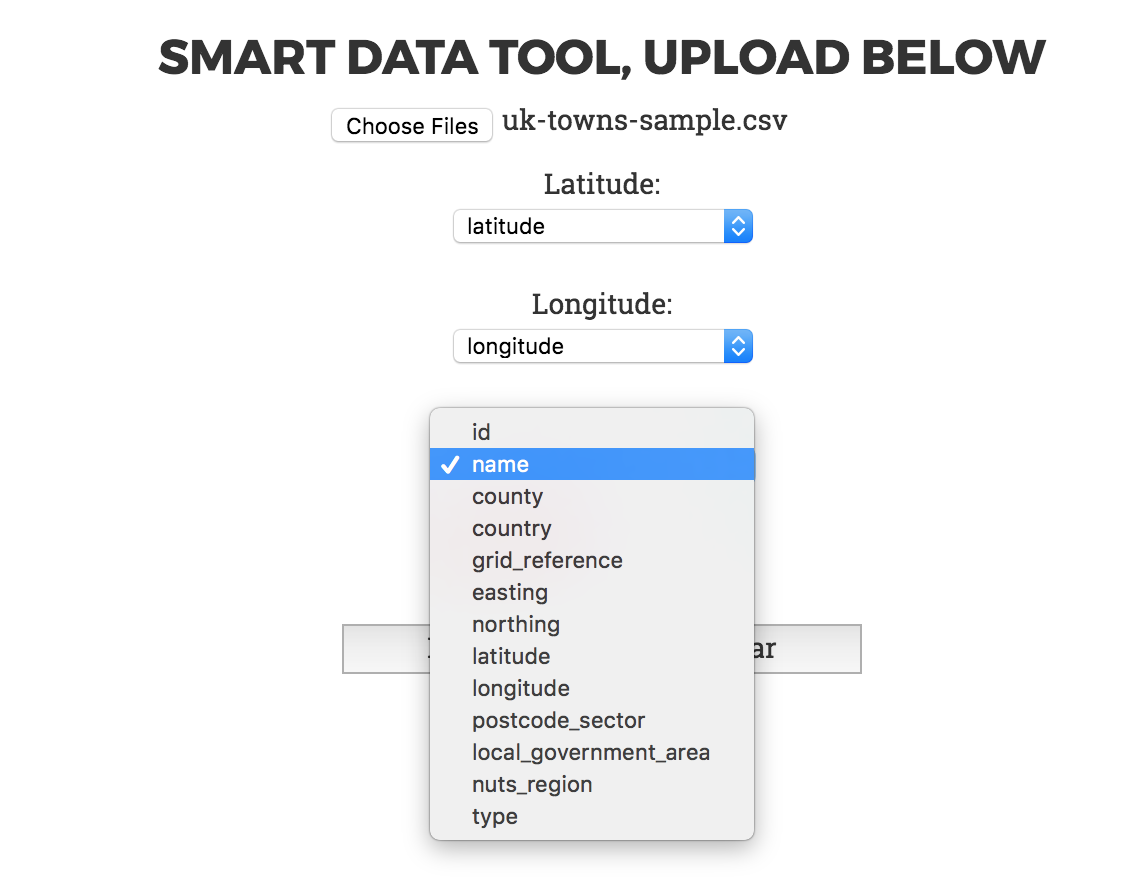
\includegraphics[width=0.4\textwidth]{sdt15}
\caption{Smart Data Tool Town Example}
\label{fig:sdt}
\end{center}
\end{figure}

Figure \ref{fig:sdt2} shows the result when the uk-towns-sample.csv dataset is drawn with the allergy symptoms heatmap behind.

\begin{figure}[H]
\begin{center}
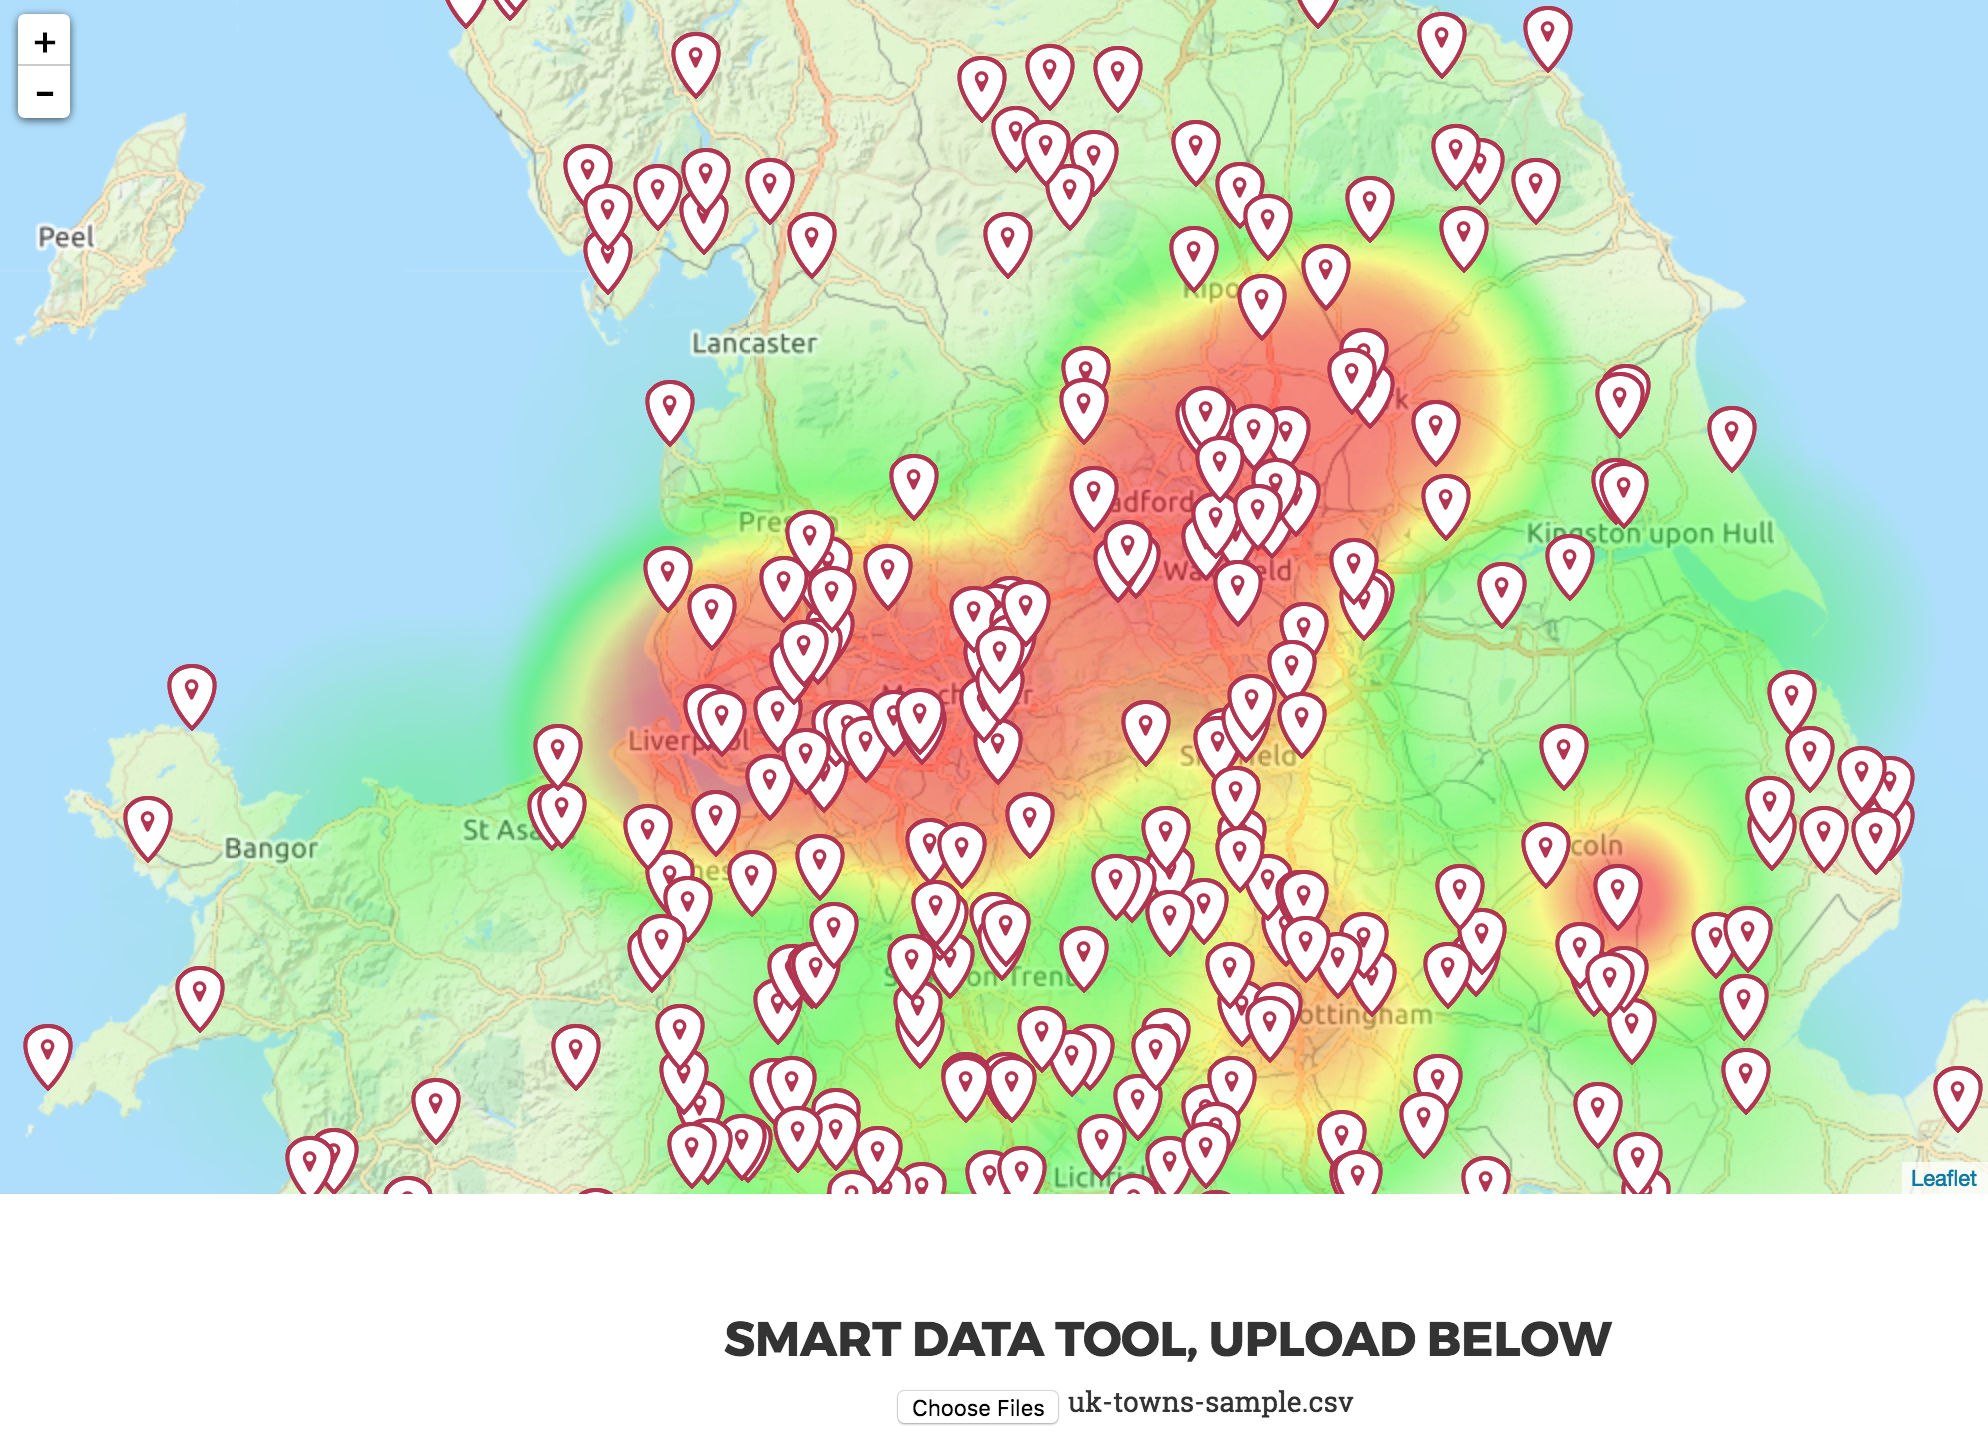
\includegraphics[width=0.4\textwidth]{sdt2}
\caption{Smart Data Tool Town Map}
\label{fig:sdt2}
\end{center}
\end{figure}